\graphicspath{{img/ch2}}

\section{Lunar Pit Geological Characteristics}

\subsection{Morphological Characteristics}

Lunar pits exhibit distinct morphological features that provide critical insights into their geological origins and evolution. They typically feature a funnel-shaped upper region leading into near-vertical walls, often ending in flat or concave floors \cite{new-wagner}. The sharp transition between the sloping entrance and vertical walls suggests sudden roof collapse above a subsurface void, rather than gradual erosion processes \cite{lunar-pits-numerical-modelling, lunar-pits-entrances-to-caves}.

\begin{figure}[h!]
    \centering
    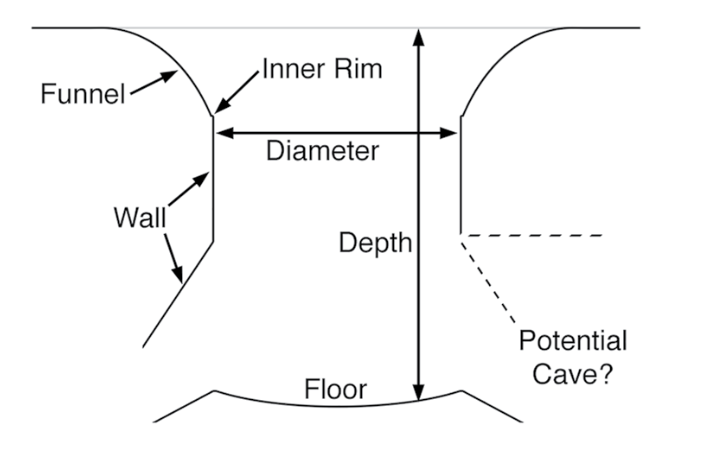
\includegraphics[width=0.5\linewidth]{lunar_pit_schema.png}
    \caption{A simplified schematic of a generic lunar pit cross-section showing key morphological features (adapted from \cite{new-wagner}).}
    \label{fig:lunar-pit-schema}
\end{figure}

High-resolution images from the Lunar Reconnaissance Orbiter (LRO) Narrow Angle Camera (NAC) have revealed significant details, such as layering within pit walls. These layers, likely corresponding to successive volcanic flow events, provide a geological record of ancient lunar volcanism \cite{new-wagner}. Observations of overhangs within pits, particularly at Marius Hills and Mare Tranquillitatis, suggest access to extensive subsurface voids, often interpreted as collapsed lava tubes \cite{lunar-pits-entrances-to-caves, Carrer2024}. These voids could be tens of meters in length and offer compelling targets for future exploration \cite{lava-tube-observations}.

The base of lunar pits typically contains accumulations of boulders and regolith. Some pits exhibit concave floors, contributing significantly to their depth and distinguishing them from traditional impact craters, which feature raised rims and ejecta blankets \cite{new-wagner}.

\begin{figure}[H]
    \centering
    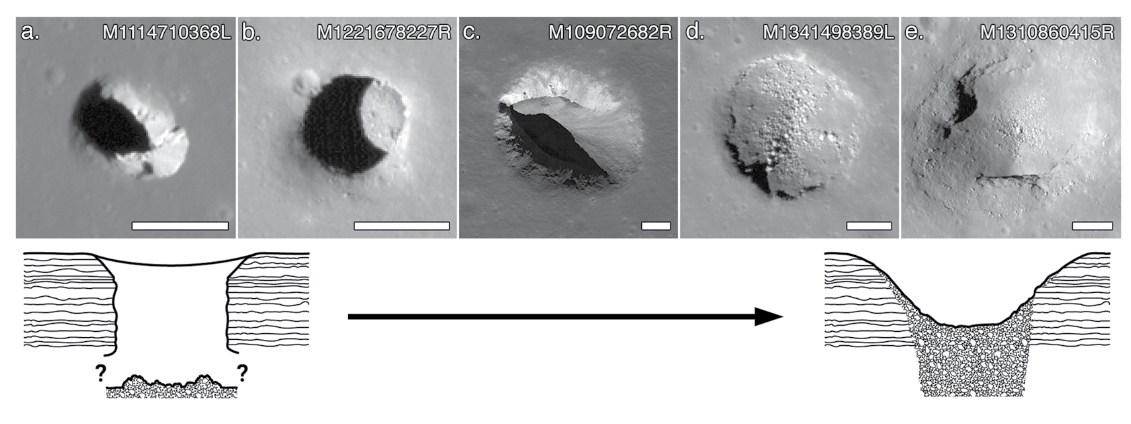
\includegraphics[width=0.85\linewidth]{closed_and_open_cavities.png}
    \caption{Progression of lunar pit degradation, illustrating gradual erosion and regolith deposition over time. Figure shows different lunar pits in various stages of erosion (adapted from \cite{new-wagner}).}
    \label{fig:lunar-pit-degradation}
\end{figure}

Over geological timescales, lunar pits degrade due to micrometeoroid impacts, thermal cycling, and seismic activity. These processes erode walls and rims, depositing debris at the base. Some pits, such as those in Mare Tranquillitatis and Marius Hills, show varying states of preservation, with sharp walls in younger features and smoother, infilled floors in older examples \cite{lunar-pit-distribution}. The degradation process operates independently of the surrounding terrain age, suggesting pits evolve gradually over hundreds of millions of years \cite{new-wagner, lunar-pits-numerical-modelling}.

\subsection{Geographical Distribution and Formation Mechanisms}

Lunar pits are distributed across three primary geological settings: mare basalts, impact melt deposits, and highland terrain. These pits provide a unique window into the Moon's geological evolution and are formed by distinct mechanisms based on their location and context \cite{lunar-pit-distribution, lunar-pits-numerical-modelling}.

\begin{figure}[H]
    \centering
    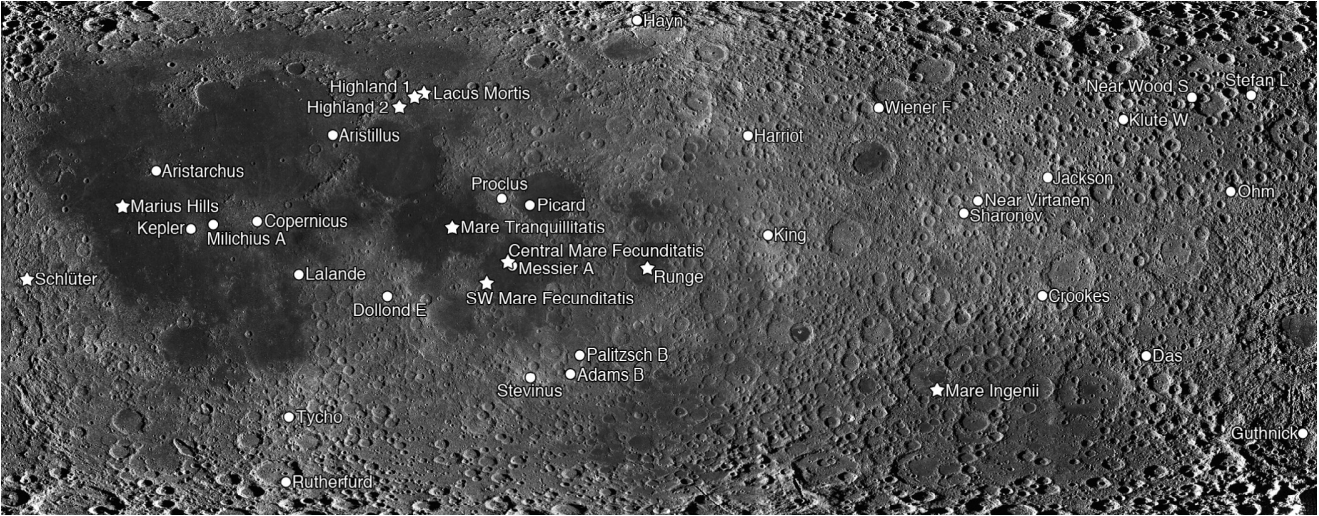
\includegraphics[width=0.76\linewidth]{map-lunar-pits-rough.png}
    \caption{Map of lunar pits: eight in mare basalts, two in highlands (stars), and 29 in impact melt deposits (dots). Figure adapted from \cite{lunar-pit-distribution}.}
    \label{fig:map-lunar-pits}
\end{figure}

\paragraph{Mare Basalts} Pits in mare regions, such as Marius Hills and Mare Tranquillitatis, are primarily linked to volcanic activity. These pits likely form due to the collapse of lava tube roofs, where thinning overlying material becomes unstable and collapses into subsurface voids \cite{lunar-pits-entrances-to-caves}. Such pits are often found near sinuous rilles, which are remnants of ancient volcanic flow channels, further indicating their volcanic origin. For instance, radar and imaging data from the Mare Tranquillitatis pit revealed an extensive subsurface void consistent with a collapsed lava tube \cite{Carrer2024, lava-tube-observations} (see \ref{fig:image1}). These features not only indicate ancient volcanic activity but also provide potential access to well-preserved lava tube interiors.

\begin{figure}[H]
    \centering
    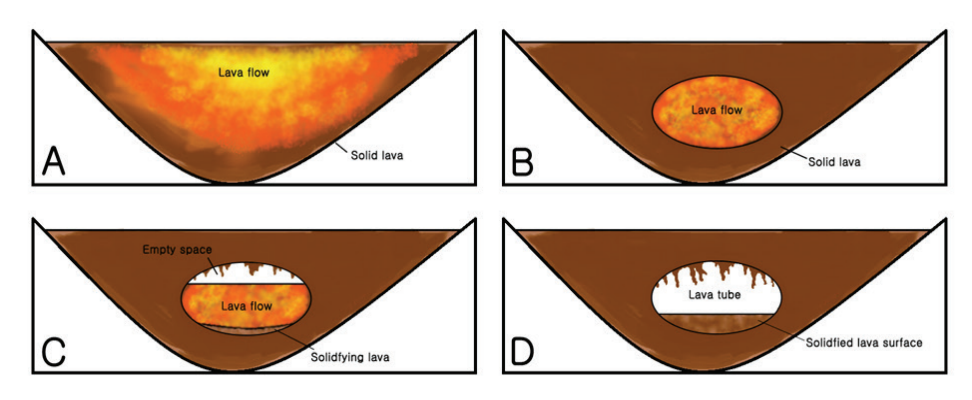
\includegraphics[width=0.7\linewidth]{lava_tube_formation_schema.png}
    \caption{Stages of lunar lava tube formation, illustrating crust solidification, lava drainage, and resulting voids (adapted from \cite{lunar-pits-entrances-to-caves}).}
    \label{fig:lava-tube-formation-schema}
\end{figure}

\paragraph{Impact Melt Deposits} Pits found within younger impact craters, such as Tycho and Copernicus, form due to a combination of impact-generated processes. High-energy impacts fracture and compress the lunar crust while generating immense heat that melts surface and subsurface material. This molten impact melt redistributes across the crater floor, forming pools of rapidly cooling material. During solidification, thermal contraction creates extensive cracks and fractures \cite{new-wagner}. Simultaneously, void spaces can develop where molten material drains or collapses into pre-existing subsurface cavities. Over time, localized collapses along these fractures or voids form impact melt pits \cite{lunar-pits-numerical-modelling, lunar-pit-distribution}. Unlike volcanic pits, these features are typically more circular in shape, lack overhangs, and show no association with lava flows.

\begin{figure}[H]
    \centering
    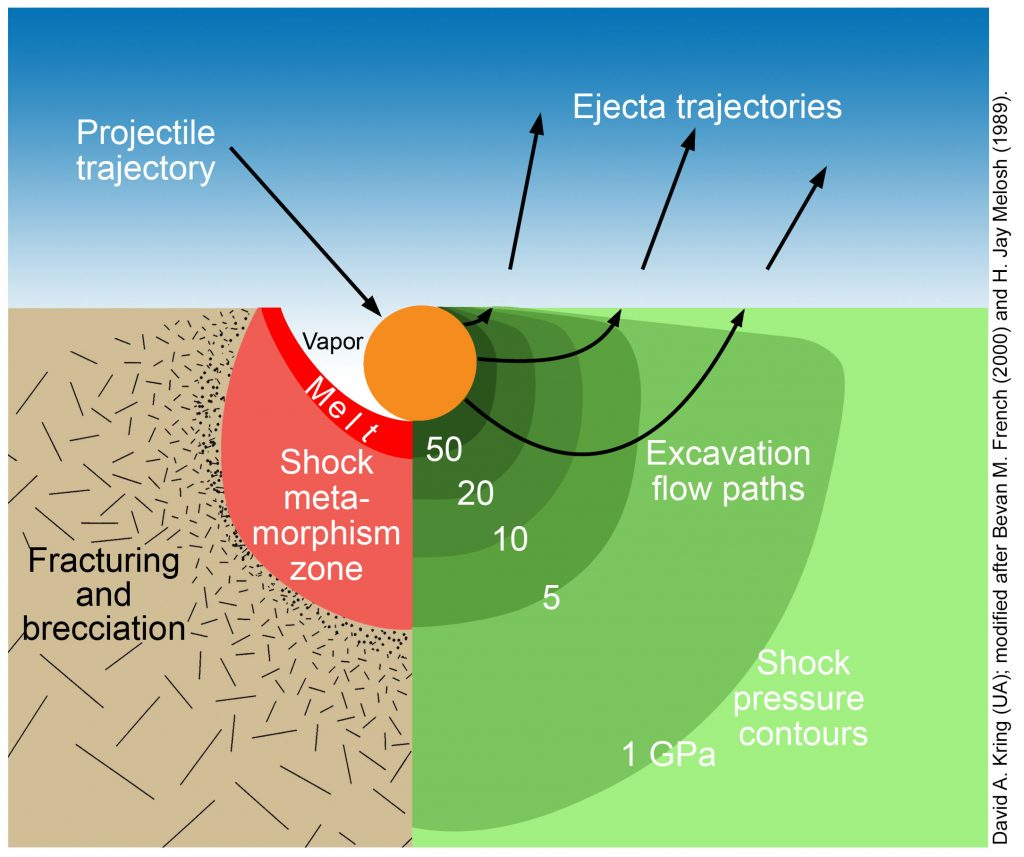
\includegraphics[width=0.42\linewidth]{Impact-Shock-Pressures-and-Their-Effects-1024x857.jpg}
    \caption{Impact dynamics illustrating pressure zones, molten material, formation of cracks, contributing to pit formation in impact melt deposits (adapted from     \cite{clrn-impact-melt}).}
    \label{fig:impact-melt}
\end{figure}

\paragraph{Highland Terrain} Highland pits are rare and thought to result from tectonic stress and extensional faulting. These pits typically form near large-scale graben systems or faulted regions, where crustal stress generates fractures in the lunar surface. Over time, localized collapse along these fault zones forms pits with sharp, near-vertical walls \cite{new-wagner}. Examples include the Lacus Mortis pit and pits in the Rima Hyginus region, which are situated along prominent grabens. Unlike mare pits, highland pits lack volcanic features or associations with lava tubes, making their tectonic origins more evident \cite{lunar-pit-distribution}.

\begin{figure}[H]
    \centering
    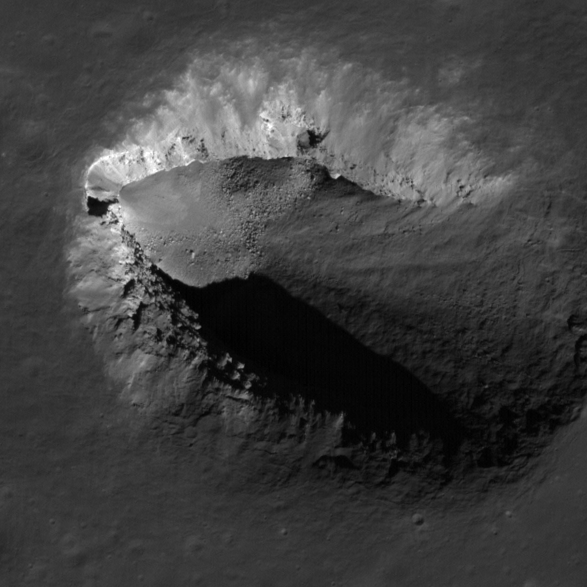
\includegraphics[width=0.33\linewidth]{lunar-pit-highland.png}
    \caption{Lunar Reconnaissance Orbiter Camera footage of Lacus Mortis Pit. Image adapted from: \url{https://www.lroc.asu.edu/atlases/pits}.}
    \label{fig:highland-lunar-pit}
\end{figure}

\paragraph{Impact-Induced Skylights}form when small meteoroid impacts trigger the collapse of thin crusts overlying intact subsurface voids, such as lava tubes. Unlike traditional impact craters, these skylights lack ejecta blankets and raised rims because the impact energy is localized and primarily directed toward destabilizing the roof material \cite{lunar-pits-numerical-modelling}.

For example, the Marius Hills pit provides a compelling case: numerical models suggest that a meteoroid impact on a 26-meter-thick roof caused its collapse, forming a skylight approximately 40 meters in diameter. The underlying void remained intact, but the shock wave and resulting fractures weakened the overlying material enough to cause it to cave in \cite{clrn-impact-melt}.

\begin{figure}[H]
    \centering
    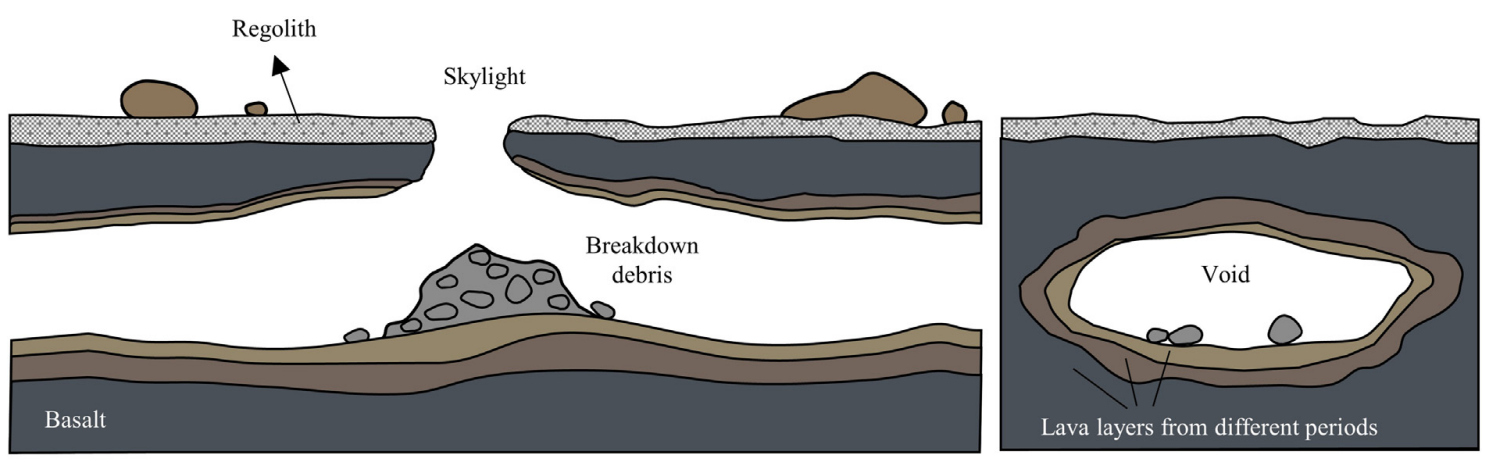
\includegraphics[width=0.99\linewidth]{lunar-pit-in-lava-tube.png}
    \caption{Cross section of a lunar tube with collapsed skylight (adapted from    \cite{bases-feng}).}
    \label{fig:impact-induced-skylight}
\end{figure}
